\section{Steepest Descent}

Let's now finally explore integrals over the complex plane with complex valued functions. We retake the integral 
\begin{equation}
	\phi(\lambda) := \int_{\Gamma} g(s) \ee^{-\lambda f(s)} \dd s,
	\label{eq: general int}
\end{equation}
where $\Gamma$ is a contour in the complex plane and $f, g$ are given \textit{complex-valued, analytic functions.}

Suppose that $\Gamma$ is parametrized by $\gamma : [a,b] \rightarrow \C$ and let us decompose the functions we have into their real and imaginary parts such as
$$f(z) = u(z) + \ii v(z), \ \ g(z) = p(z) + \ii q(z), \ \ \gamma(t) = \alpha(t) + \ii \beta(t)$$
with all functions in the decomposition being real valued. Of course we now have 
$$\ee^{-\lambda f(z)} = \ee^{-\lambda u(z)} \ee^{-\ii v(z)}$$
and when $\lambda$ grows large, we have the exponentially growing/decaying term $\ee^{-\lambda u(z)}$ and a oscillating term coming from $\ee^{\ii v(z)}$ which is hard to control. The idea to get around this fact is to use paths in which this term is constant. If we have such a case, we would write

\begin{equation}
	\Phi(\lambda) = \ee^{-\ii \lambda v_0} \int_{a}^{b} (p(\gamma(t))\alpha'(t)-q(\gamma(t))\beta'(t)) \ee^{-\lambda u(\gamma(t))} \dd t + \ii \ee^{-\ii \lambda v_0} \int_{a}^{b} (p(\gamma(t))\beta'(t)-q(\gamma(t))\alpha'(t)) \ee^{-\lambda u(\gamma(t))} \dd t
	\label{eq: decomposition}
\end{equation}
where each integral can now be solved by Laplace's method.

\begin{thm}
	Consider $\Phi$ as in \ref{eq: general int} with a smooth contour $\Gamma$. Assume that the exponent $f = u + \ii v$ is an analytic function on a neighborhood of $\Gamma$ that satisfies
	$$v(z) \equiv v_0, \ \ \ z \in \Gamma$$
	In addition, suppose that $u$ has a unique minimum at an interior point of $\Gamma$, say on $z_0 \in \Gamma$, with $f''(z_0) \neq 0$, and also that $g$ is analytic on a neighborhood of $\Gamma$  and satisfies
	$$\int_{\Gamma} |g(z)| |dz| < \infty.$$
	Then $\Phi$ has a leading asymptotic as $\lambda \rightarrow +\infty$ given by
	$$\Phi(\lambda) = \ee^{-\lambda f(z_0)} \left(\frac{\sqrt{2\pi}g(z_0)\ee^{\ii \theta(z_0)}}{\lambda^{1/2}\sqrt{|f''(z_0)|}} + \Boh(\lambda^{-3/2}) \right), \ \ \lambda \rightarrow + \infty,$$
	where $\theta(z_0)$ is the angle of the oriented tangent of $\Gamma$ at $z_0$.
\end{thm}

\begin{Mproof}
	Fix a parametrization $\gamma : [a,b] \rightarrow \C$ of $\Gamma$ with $\gamma(c) = z_0, a < c < b$, and decompose $\Phi$ as before in $\ref{eq: decomposition}$. By the assumptions on the functions $f, g$ we can apply Laplace`s method on both equations, and yields, as $\lambda \rightarrow + \infty$,
	$$\int_{a}^{b} (p(\gamma(t))\alpha'(t)-q(\gamma(t))\beta'(t)) \ee^{-\lambda u(\gamma(t))} \dd t = \sqrt{2\pi} \ee^{-\lambda u(z_0)} \left( \frac{p(z_0)\alpha'(c)-q(z_0)\beta'(c)}{\sqrt{|(u \circ \gamma)''(c)|} \lambda^{1/2}} + \Boh \left(\lambda^{3/2}\right) \right)$$
	and
	$$\int_{a}^{b} (p(\gamma(t))\beta'(t)-q(\gamma(t))\alpha'(t)) \ee^{-\lambda u(\gamma(t))} \dd t = \sqrt{2\pi} \ee^{-\lambda u(z_0)} \left( \frac{p(z_0)\beta'(c)-q(z_0)\alpha'(c)}{\sqrt{|(u \circ \gamma)''(c)|} \lambda^{1/2}} + \Boh \left(\lambda^{3/2}\right) \right)$$
	Using that $v_0 + u(z_0) = f(z_0)$ and also that,
	$$ (p(z_0)\alpha'(c)-q(z_0)\beta'(c)) + \ii (p(z_0)\beta'(c)-q(z_0)\alpha'(c)) = g(z_0)\gamma'(c).$$
	Combining the estimative for both parts we get
	$$\Phi(\lambda) = \sqrt{2\pi} \ee^{-\lambda f(z_0)} \left( \frac{g(z_0)\gamma'(c)}{\sqrt{|(u \circ \gamma)''(c)|} \lambda^{1/2}} + \Boh \left(\lambda^{3/2}\right) \right)$$ 
	and it suffices now to get an expression for the second derivative in the denominator. Knowing the imaginary part is constant we can write
	$$\frac{\dd}{\dd t} u(\gamma(t)) = \frac{\dd}{\dd t} f(\gamma(t)) = \gamma'(t) f'(\gamma(t))$$
	and
	$$ \frac{\dd^2}{\dd t} u(\gamma(t)) = \frac{\dd^2}{\dd t} f(\gamma(t)) = (\gamma'(t))^2 f''(\gamma(t)) + \gamma''(t) f'(\gamma(t)).$$
	Hence,
	$$ \frac{\gamma'(c)}{\sqrt{|(u \circ \gamma)''(c)|}} = \frac{1}{\sqrt{|f''(z_0)|}} \frac{\gamma'(c)}{|\gamma'(c)|}$$
	which concludes the proof.
\end{Mproof}

We now need do discuss why this assumption of constant value of $\Im(f(z))$ is not an assumption as strong as one might assume at first. Suppose we want to integrate in a random contour $\Gamma$ of the plane. Of course, our assumption that the functions were analytic permit us to deform the contour keeping the value of the integral. We are going to use this to find an contour $\tilde{\Gamma}$ such that sections of the contour are such that $\Im(f(z))$ is constant. in the figure above we plot such a scenario by using the level lines of the imaginary part of $f$ as curves on the plane. 

\begin{figure}[h]
	\centering
	\subfigure{
		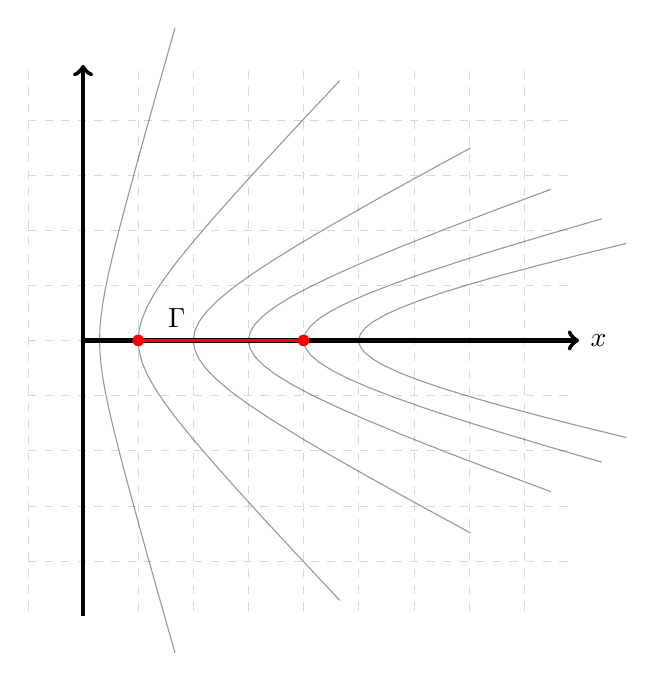
\begin{tikzpicture}[scale=.7]
			\draw[help lines, color=gray!30, dashed] (-1,-4.9) grid (8.9,4.9);
			\draw[->,ultra thick] (0,0)--(9,0) node[right]{$x$};
			\draw[->,ultra thick] (0,-5)--(0,5) node[above]{$\ii$};
			\pgfmathsetmacro{\e}{1.44022}   % eccentricity
			\pgfmathsetmacro{\a}{1}
			\pgfmathsetmacro{\b}{(\a*sqrt((\e)^2-1)} 
			\draw[opacity=0.4] plot[domain=-2.4:2.4] ({0.3*\a*cosh(\x)},{\b*sinh(\x)});
			\draw[opacity=0.4] plot[domain=-2.22:2.22] ({1*\a*cosh(\x)},{\b*sinh(\x)});
			\draw[opacity=0.4] plot[domain=-1.93:1.93] ({2*\a*cosh(\x)},{\b*sinh(\x)});
			\draw[opacity=0.4] plot[domain=-1.7:1.7] ({3*\a*cosh(\x)},{\b*sinh(\x)});
			\draw[opacity=0.4] plot[domain=-1.5:1.5] ({4*\a*cosh(\x)},{\b*sinh(\x)});
			\draw[opacity=0.4] plot[domain=-1.3:1.3] ({5*\a*cosh(\x)},{\b*sinh(\x)});
			\node (Gamma) at (1.7,0.4)    {$\Gamma$};
			\draw[color=red, very thick] (1,0) -- (4,0);
			\fill[color=red] (1,0) circle (3pt);
			\fill[color=red] (4,0) circle (3pt);
		\end{tikzpicture}
	}
	\subfigure{
		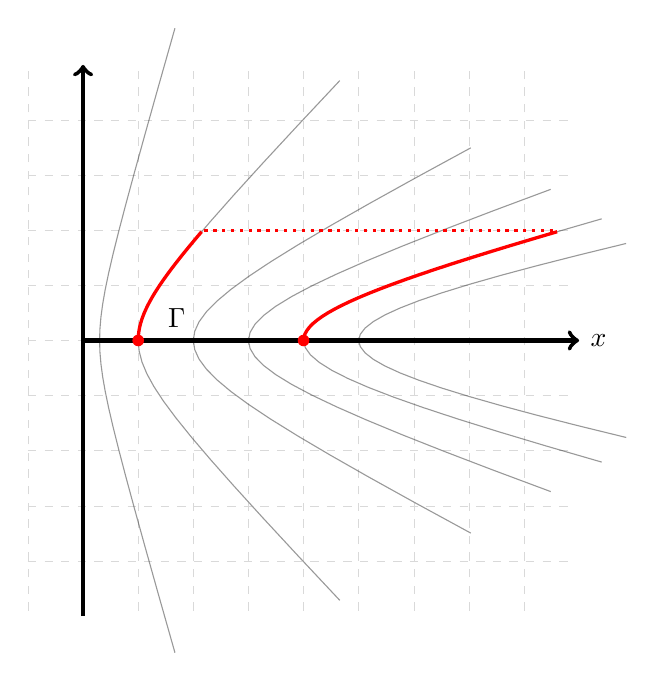
\begin{tikzpicture}[scale=.7]
			\draw[help lines, color=gray!30, dashed] (-1,-4.9) grid (8.9,4.9);
			\draw[->,ultra thick] (0,0)--(9,0) node[right]{$x$};
			\draw[->,ultra thick] (0,-5)--(0,5) node[above]{$\ii$};
			\pgfmathsetmacro{\e}{1.44022}   % eccentricity
			\pgfmathsetmacro{\a}{1}
			\pgfmathsetmacro{\b}{(\a*sqrt((\e)^2-1)} 
			\draw[opacity=0.4] plot[domain=-2.4:2.4] ({0.3*\a*cosh(\x)},{\b*sinh(\x)});
			\draw[opacity=0.4] plot[domain=-2.22:2.22] ({1*\a*cosh(\x)},{\b*sinh(\x)});
			\draw[opacity=0.4] plot[domain=-1.93:1.93] ({2*\a*cosh(\x)},{\b*sinh(\x)});
			\draw[opacity=0.4] plot[domain=-1.7:1.7] ({3*\a*cosh(\x)},{\b*sinh(\x)});
			\draw[opacity=0.4] plot[domain=-1.5:1.5] ({4*\a*cosh(\x)},{\b*sinh(\x)});
			\draw[opacity=0.4] plot[domain=-1.3:1.3] ({5*\a*cosh(\x)},{\b*sinh(\x)});
			\node (Gamma) at (1.7,0.4)    {$\Gamma$};
			
			\draw[color=red, very thick] plot[domain=0:1.4] ({1*\a*cosh(\x)},{\b*sinh(\x)});
			\draw[color=red, very thick] plot[domain=0:1.4] ({4*\a*cosh(\x)},{\b*sinh(\x)});
			\draw[color=red, very thick, dotted] (2.2,2) -- (8.6,2);
			
			\fill[color=red] (1,0) circle (3pt);
			\fill[color=red] (4,0) circle (3pt);
		\end{tikzpicture}
	}
\end{figure}

The name given by the method is also intuitive. We already know that being analytic means satisfying the \textit{Cauchy-Riemann} equations,
$$u_x(z) = v_y(z), \ \text{and} \ \ u_y(z) = -v_x(z).$$
An immediate result from these equation is that the gradients of $u$ and $v$ must be normal. Indeed, if $<\cdot, \cdot>$ is the inner product on $\R^2$,
$$<\nabla u(z), \nabla v(z) > = u_x(z)v_x(z) + u_y(z)v_y(z) = u_x(z)v_x(z) - v_x(z)u_x(z) = 0.$$
As we're following the curves where  $\Im(f(z))$ is constant, we're also following the path of \textit{steepest descent} of the real part of the integral. As we also are looking to use Laplace's method on the integrals, we may want to have our paths going through the critical points of the function.